\subsection{Hash Map}
\definecolor{inkscapeNavy}{rgb}{0.0, 0.0, 0.5}
\definecolor{inkscapeGreen}{rgb}{0.0, 0.5, 0.0}
\definecolor{inkscapeMaroon}{rgb}{0.5, 0.0, 0.0}

\begin{frame}{Associative Arrays}{The Hash Map}
  \textbf{Idea:}
  \begin{itemize}
    \item
      Mapping the keys onto indices with a {\color{MainA}hash function}
    \item
      Store the values at the calculated indices in a normal array
  \end{itemize}
  \textbf{Example:}
  \begin{itemize}
    \item
      Key set: $x = \{3904433, 312692, 5148949\}$
    \onslide <2-> \item
      Hash function:
      {\color{MainA}$h(x) = x \;\mathrm{mod}\; 5$},
      in the range {\color{MainA} $[0, \ldots, 4]$ }
    \onslide <3-> \item We need an array {\color{MainA}T}
      with {\color{MainA}5} elements.\\
      A \enquote{hash table} with 5 \enquote{buckets}
    \onslide <4-> \item
      The element with the key {\color{MainA}x}
      is stored in {\color{MainA}$T[h(x)]$}
  \end{itemize}
\end{frame}

%-------------------------------------------------------------------------------

\begin{frame}{Associative Arrays}{The Hash Map}
  \textbf{Storage:}
  \vspace{0.1em}
  \begin{itemize}
    \setlength\itemsep{0.75em}
    \item<2->
    \small \texttt{insert(3904433,"A")}:
    $h(3904433) = 3 \hspace*{-0.1em} \Rightarrow$
    T[3] = {\color{inkscapeGreen}(3904433, "A")}
    \item<3->
    \small \texttt{insert(312692, "B")}:
    $h(312692) = 2 \hspace*{-0.1em} \Rightarrow$
    T[2] = {\color{inkscapeMaroon}(312692, "B")}
    \item<4->
    \small \texttt{insert(5148949, "C")}:
    $h(5148949) = 4 \hspace*{-0.1em} \Rightarrow$
    T[4] = {\color{inkscapeNavy}(5148949, "C")}
  \end{itemize}
  \vspace{0.1em}
  \begin{figure}
  \caption{Hash table T}
  \centering
\only<1-1>{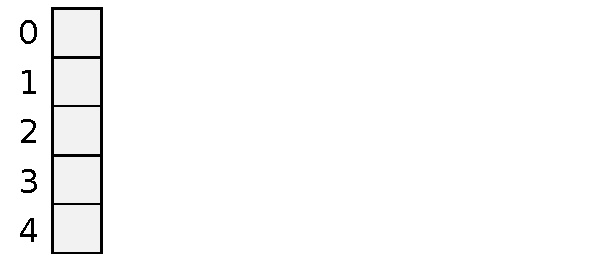
\includegraphics[width=0.6\textwidth]{Images/Bucket1.pdf}}%
\only<2-2>{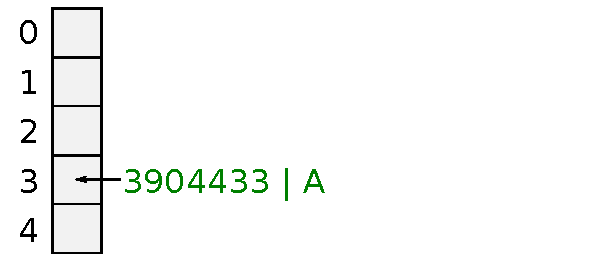
\includegraphics[width=0.6\textwidth]{Images/Bucket2.pdf}}%
\only<3-3>{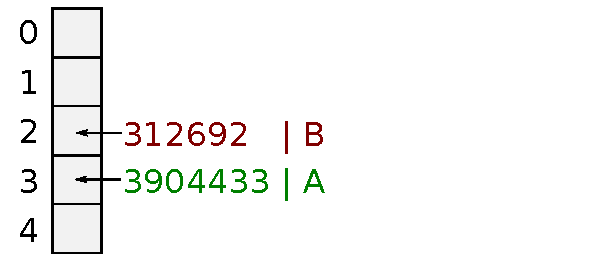
\includegraphics[width=0.6\textwidth]{Images/Bucket3.pdf}}%
\only<4->{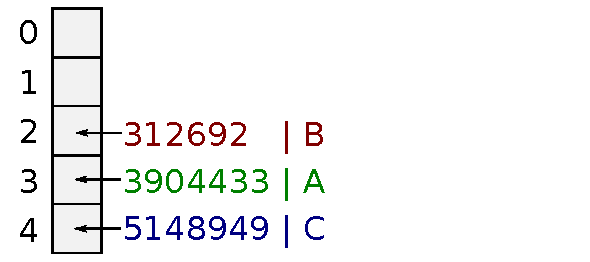
\includegraphics[width=0.6\textwidth]{Images/Bucket4.pdf}}
  \end{figure}
\end{frame}

%-------------------------------------------------------------------------------

%%%%% : TODO: Add the check step!
\begin{frame}{Associative Arrays}{The Hash Map}
  \textbf{Searching:}
  \small
  \begin{itemize}
     \setlength\itemsep{0.75em}
    \item<1->
      \texttt{search(3904433)}:
      $h(3904433) = 3 \hspace*{0.5em} \Rightarrow$
      T[3] $\rightarrow$ {\color{inkscapeGreen}(3904433, "A")}
    \item<2->
      \texttt{search(123459)}:
      $h(123459) = 4 \hspace*{0.5em} \Rightarrow$
      T[4] {}\\
      \vspace{0.75em}
      $\Rightarrow$ {\color{red}Value with key 123459 does not exist}
    \item<3->
      Search time for this example: {\color{MainA}$\mathcal{O}(1)$}
  \end{itemize}
  \vspace*{-1.0em}
  \begin{figure}
    \caption{Hash table T}
    \centering
    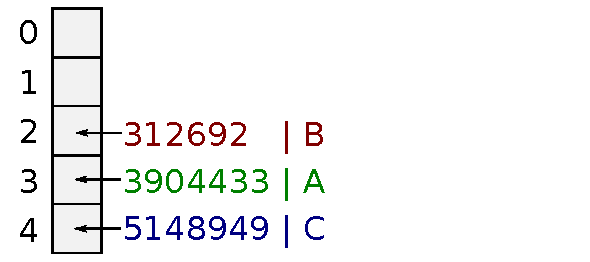
\includegraphics[width=0.6\textwidth]{Images/Bucket4.pdf}
  \end{figure}
\end{frame}

%-------------------------------------------------------------------------------

\begin{frame}{Associative Arrays}{Hash Collisions}
  \textbf{Further inserting:}
  \begin{itemize}
    \item<1->
      \texttt{insert(876543, "D")}:
      $\hspace*{0.5em} h(876543) = 3$\\
      \onslide <2->
      $\hspace*{0.5em} \Rightarrow$
      T[3] = (876543, "D")
      $\Rightarrow$ {\color{red}{Collision}}
    \item<3->
      This happens more often than expected
      \begin{itemize}
        \item
          \textbf{Birthday problem:}
          With 23 people we have the probability of $50\;\%$ that 2 of
          them have birthday at the same day
      \end{itemize}
  \end{itemize}
  \vspace*{-1.0em}
  \onslide <1->
  \begin{figure}
    \caption{Hash table T}
    \centering
       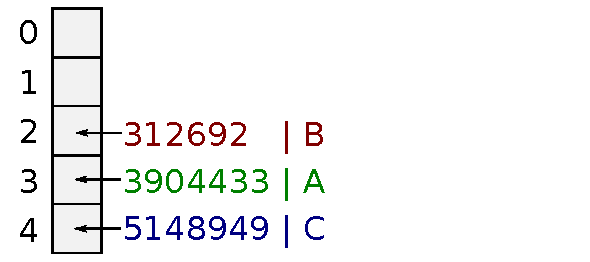
\includegraphics[width=0.6\textwidth]{Images/Bucket4.pdf}
  \end{figure}
\end{frame}

%-------------------------------------------------------------------------------

\begin{frame}{Associative Arrays}{Hash Collisions}
  \textbf{Problem:}
  \begin{itemize}
    \item
      Two keys are equal {\color{MainA} $h(x) = h(y)$} but not the values
      {\color{MainA} $x \neq y$}
  \end{itemize}
  \onslide<2->{\textbf{Easiest Solution:}}
  \begin{itemize}
    \item<3->
      Represent each bucket as list of key-value pairs
    \item<4->
      Append new values to the end of the list
  \end{itemize}
    \vspace*{-1.0em}
    \begin{figure}
    \onslide <3->\caption{Hash table T}
    \centering
    \only<1-3>{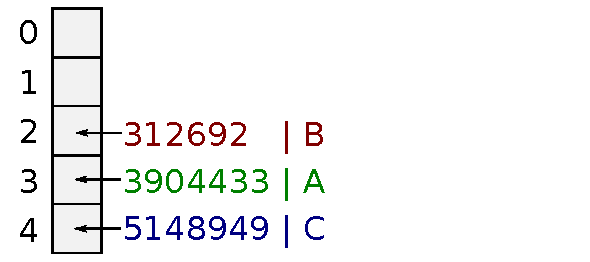
\includegraphics[width=0.6\textwidth]{Images/Bucket4.pdf}}
    \only<4-4>{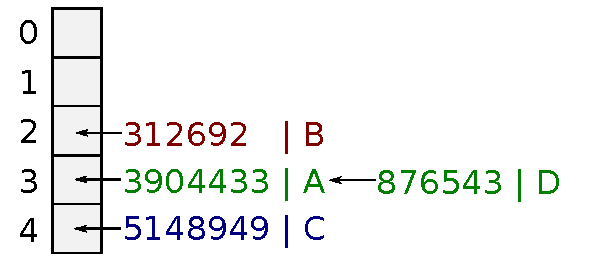
\includegraphics[width=0.6\textwidth]{Images/Bucket5.pdf}}
  \end{figure}
\end{frame}


%-------------------------------------------------------------------------------

%% \begin{frame}{Associative Arrays}{Hash Collisions}
%%   \textbf{Example:}
%%   \begin{itemize}
%%     \item
%%     Key set: $k = \{3904, 3126, 5148, 4522\}$
%%     \item
%%     Hash function:
%%     $h(k) = k \;\mathrm{mod}\; 5 \hspace*{1.0em} \in \{0, \ldots, 4\}$
%%   \end{itemize}
%%   \textbf{Inserting:}
%%   \begin{itemize}
%%     \item
%%       \dots
%%     \item
%%       \lstinline[
%%         language=Python,
%%         style={python-idle-code},
%%         basicstyle=\small
%%       ]|insert(8769, "D")|:
%%       $\hspace*{0.5em} h(8769) = 4$
%%       $\hspace*{0.5em} \Rightarrow$
%%       \lstinline[
%%         language=Python,
%%         style={python-idle-code},
%%         basicstyle=\small
%%       ]|T[4].append((8769, "D"))|
%%     \item
%%       \lstinline[
%%         language=Python,
%%         style={python-idle-code},
%%         basicstyle=\small
%%       ]|search(8769)|:
%%       $\hspace*{0.5em} h(8769) = 4$\\
%%       $\hspace*{1.5em} \Rightarrow$
%%       \lstinline[
%%         language=Python,
%%         style={python-idle-code},
%%         basicstyle=\small
%%       ]|T[4]|
%%       $\Rightarrow$
%%       \lstinline[
%%         language=Python,
%%         style={python-idle-code},
%%         basicstyle=\small
%%       ]|[(3904, "A"), (8769, "D")]|
%%   \end{itemize}
%%   \vspace*{-1.0em}
%%   \begin{table}[!b]
%%     \caption{Hash table T}
%%     \label{tab:hash_table:example_linked}
%%     \begin{tabularx}{\textwidth}{l|ccccc}
%%       {} & 0 & 1 & 2 & 3 & 4\\
%%       \midrule
%%       Bucket &
%%       \lstinline[
%%         language=Python,
%%         style={python-idle-code},
%%         basicstyle=\small
%%       ]|[]| &
%%       \lstinline[
%%         language=Python,
%%         style={python-idle-code},
%%         basicstyle=\small
%%       ]|[(3126, "B")]| &
%%       \lstinline[
%%         language=Python,
%%         style={python-idle-code},
%%         basicstyle=\small
%%       ]|[]| &
%%       \lstinline[
%%         language=Python,
%%         style={python-idle-code},
%%         basicstyle=\small
%%       ]|[(5148, "C")]| &
%%       \begin{math}
%%         \left[\begin{array}{@{}l@{}}
%%           \lstinline[
%%             language=Python,
%%             style={python-idle-code},
%%             basicstyle=\small
%%           ]|(3904, "A"),|\\
%%           \lstinline[
%%             language=Python,
%%             style={python-idle-code},
%%             basicstyle=\small
%%           ]|(8769, "D")|
%%         \end{array}\right]
%%       \end{math}
%%     \end{tabularx}
%%   \end{table}
%% \end{frame}

%-------------------------------------------------------------------------------

\begin{frame}{Associative Arrays}{Expected Runtime}
  \begin{columns}
    \begin{column}{0.5\linewidth}
      {\color{MainA}Best case}:
      \begin{itemize}
        \item
          We have {\color{MainA}$n$} keys which are equally distributed over {\color{MainA}$m$} buckets
        \item
          We have {\color{MainA}$\approx \frac{n}{m}$} pairs per bucket
        \item
          The runtime for searching is nearly {\color{MainA}$\mathcal{O}(1)$}
          if \textbf{not} {\color{MainA}$n \gg m$}
      \end{itemize}
    \end{column}
    \begin{column}{0.5\linewidth}
      \begin{center}
        \textbf{Best case}\\
        \textbf{($m = 5, \, n = 10$)}\\[1em]
        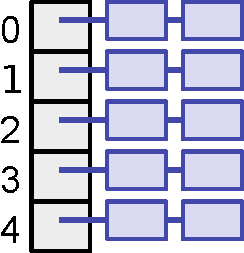
\includegraphics[height=0.4\textheight]{Images/hash-uniform.pdf}
%        \label{tab:hash_table:runtime_best_case}
        %  \begin{tabularx}{\textwidth}{c|c}
        %   {} & Bucket\\
        %   \midrule
        %   0 & \lstinline[
        %     language=Python,
        %     style={python-idle-code},
        %     basicstyle=\small,
        %     mathescape
        %   ]|[($\ldots$), ($\ldots$)]|\\
        %   1 & \lstinline[
        %     language=Python,
        %     style={python-idle-code},
        %     basicstyle=\small,
        %     mathescape
        %   ]|[($\ldots$), ($\ldots$)]|\\
        %   2 & \lstinline[
        %     language=Python,
        %     style={python-idle-code},
        %     basicstyle=\small,
        %     mathescape
        %   ]|[($\ldots$), ($\ldots$)]|\\
        %   3 & \lstinline[
        %     language=Python,
        %     style={python-idle-code},
        %     basicstyle=\small,
        %     mathescape
        %   ]|[($\ldots$), ($\ldots$)]|\\
        %   4 & \lstinline[
        %     language=Python,
        %     style={python-idle-code},
        %     basicstyle=\small,
        %     mathescape
        %   ]|[($\ldots$), ($\ldots$)]|
        % \end{tabularx}
      \end{center}
    \end{column}
  \end{columns}
\end{frame}

%-------------------------------------------------------------------------------

\begin{frame}{Associative Arrays}{Expected Runtime}
  \begin{columns}
    \begin{column}{0.4\linewidth}
      {\color{MainA}Worst case}:
      \begin{itemize}
        \item
          All {\color{MainA}$n$} keys are mapped onto the same bucket
        \item
          The runtime is {\color{MainA}$\Theta(n)$} for searching
      \end{itemize}
    \end{column}
    \begin{column}{0.5\linewidth}
      \begin{center}
        \textbf{Worst case}\\
        \textbf{($m = 5, \, n = 10$)}\\[1em]
        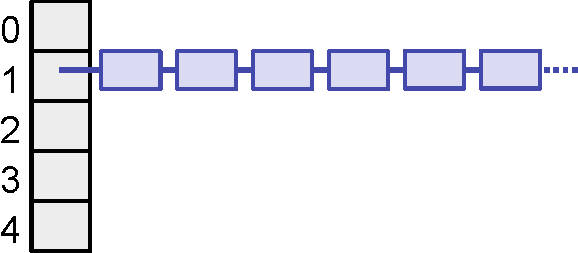
\includegraphics[height=0.4\textheight]{Images/hash-extreme.pdf}
        \label{tab:hash_table:runtime_worst_case}
        % \begin{tabularx}{\textwidth}{c|c}
        %   {} & Bucket\\
        %   \midrule
        %   0 & \lstinline[
        %     language=Python,
        %     style={python-idle-code},
        %     basicstyle=\small
        %   ]|[]|\\
        %   1 & \lstinline[
        %     language=Python,
        %     style={python-idle-code},
        %     basicstyle=\small
        %   ]|[]|\\
        %   2 & \lstinline[
        %     language=Python,
        %     style={python-idle-code},
        %     basicstyle=\small,
        %     mathescape
        %   ]|[($\ldots$), ($\ldots$), $\;\ldots\;$, ($\ldots$)]|\\
        %   3 & \lstinline[
        %     language=Python,
        %     style={python-idle-code},
        %     basicstyle=\small
        %   ]|[]|\\
        %   4 & \lstinline[
        %     language=Python,
        %     style={python-idle-code},
        %     basicstyle=\small
        %   ]|[]|
        % \end{tabularx}
      \end{center}
    \end{column}
  \end{columns}
\end{frame}

